% This file provides an example Beamer presentation using the RWTH theme
% showcasing some of the more common options, similar to the Powerpoint version
% 12.11.2014: Revision 1 (Harold Bruintjes, Tim Lange)

% For RWTH, beamer should be loaded with class option t (top)
\documentclass[t]{beamer}
%\documentclass[t,handout]{beamer}

% Use fontspec to get Arial font
% Requires use of XeLaTeX
%\usepackage{fontspec}
%\setmainfont{Arial}
%\setsansfont{Arial}
\usepackage[scaled=.90]{helvet}
%\usepackage{helvet}
% Also force Arial for math for a more consistent look
%\usepackage{unicode-math}
%\setmathfont{Arial}

% German style date formatting (footer)
%\usepackage[ddmmyyyy]{datetime}
%\renewcommand{\dateseparator}{.}

% Format the captions used for figures etc.
\usepackage[compatibility=false]{caption}
\captionsetup{singlelinecheck=off,justification=raggedleft,labelformat=empty,labelsep=none}

% PGFPlots is used for drawing some of the charts
%\usepackage{pgfplots}
%\pgfplotsset{compat=newest}
%\input{plot_commands.tex}

\usepackage[english]{babel}
\usepackage{tikz}
\usetikzlibrary{arrows.meta, positioning}

% Load the actual RWTH theme. Suggested is to load the full theme,
% as it requires some specific dimensions
\usetheme{rwth}

\setbeamercolor{math text}{fg=rwth}
\setbeamertemplate{theorems}[numbered]
\newtheorem{algorithm}[theorem]{Algorithm}

% Setup presentation information
\title{Large Language Models and Data Streams}
\subtitle{
  Seminar \textsl{Data Stream Management and Analysis}\\[1ex]
  \insertdate\\[1ex]
  \insertauthor
}
\date{\today}
\author{Silyu Li}
\institute{RWTH Aachen University}

% Set the logo to the file `logo`
% It will be scaled automatically
\logo{
\includegraphics[scale=0.6]{rwth_i5_en_rgb.pdf}}

% Uncomment this if you want a TOC at every section start
%\AtBeginSection[]{
%  \begin{frame}<beamer>{Outline}
%    \tableofcontents[currentsection]
%  \end{frame}
%}
%\AtBeginSubsection[]{
%  \begin{frame}<beamer>{Outline}
%    \tableofcontents[currentsection,currentsubsection]
%  \end{frame}
%}

% Use this to control some aspects of the footer
%\setbeamertemplate{footertextextra}{Extra text in the footer\enskip|\enskip{}Extra text in the footer}
\setbeamertemplate{footertext}{%
  \insertshorttitle\\[1ex]\insertauthor}

% Title page
\setbeamercolor{title page bar}{fg=white}
\setbeamertemplate{title page}[rwth][title_small]{}



\begin{document}
\begin{frame}[plain]
  \titlepage
\end{frame}

%\begin{frame}{Overview}
%  \tableofcontents
%\end{frame}

\section{Introduction}
\begin{frame}{Background}
  \begin{columns}
    \begin{column}{0.4\textwidth}
        \begin{figure}
            \centering
            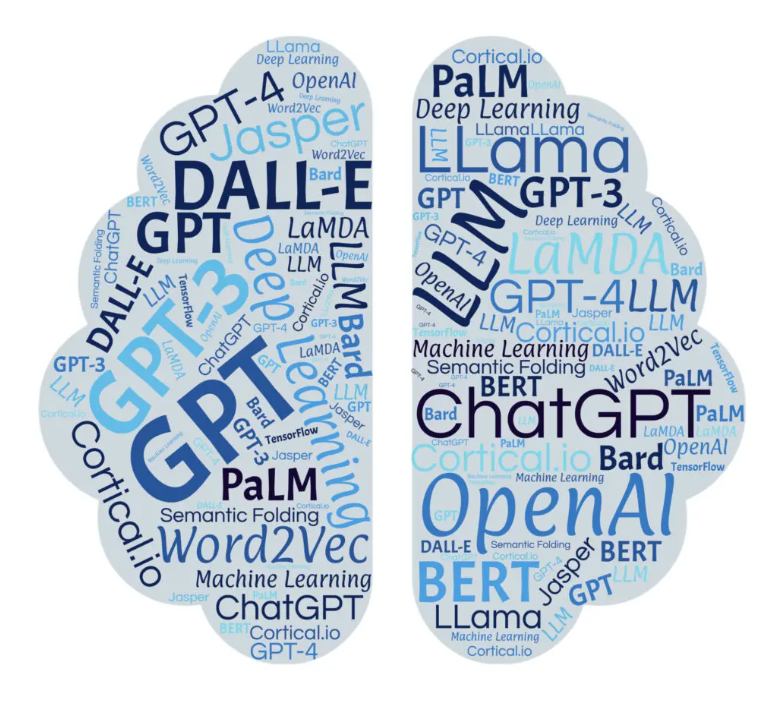
\includegraphics[width=\textwidth]{llm1.png}
            \caption{relevant concepts\footnote{Source: url{https://www.cortical.io/blog/chatgpt-and-large-language-models-the-holy-grail-of-enterprise-ai/}}}
            \label{fig:llm1}
        \end{figure}
    \end{column}
    \begin{column}{0.5\textwidth}
        \begin{itemize}
            \item LLM and AI have become very hot topics in recent years.
        \end{itemize}
    \end{column}
\end{columns}
\end{frame}

\begin{frame}{Background}
  \begin{columns}
    \begin{column}{0.4\textwidth}
        \begin{figure}
            \centering
            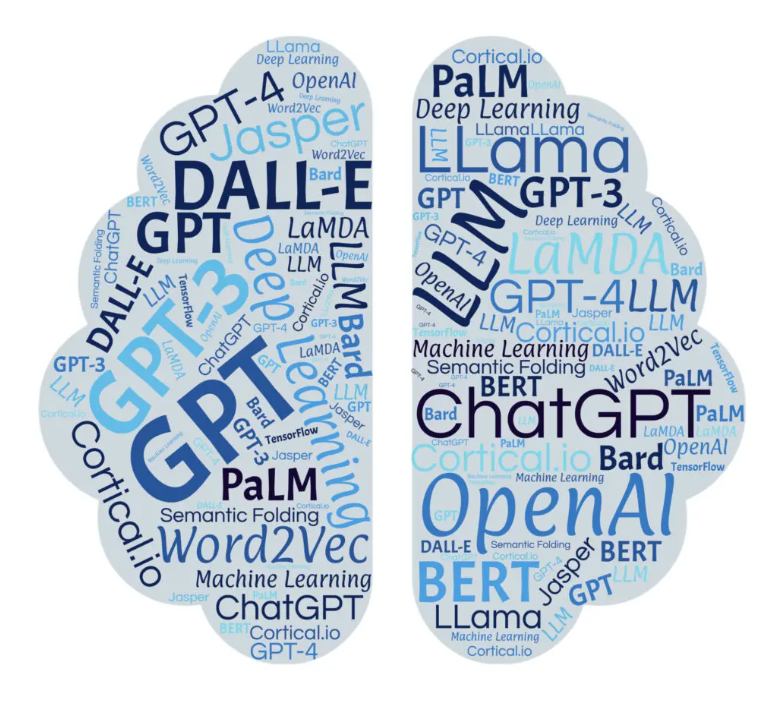
\includegraphics[width=\textwidth]{llm1.png}
            \caption{relevant concepts\footnote{Source: url{https://www.cortical.io/blog/chatgpt-and-large-language-models-the-holy-grail-of-enterprise-ai/}}}
            \label{fig:llm1}
        \end{figure}
    \end{column}
    \begin{column}{0.5\textwidth}
        \begin{itemize}
            \item LLM and AI have become very hot topics in recent years.
            \item Various models have shown their wide usage and significant competence in many fields.
        \end{itemize}
    \end{column}
\end{columns}
\end{frame}

\begin{frame}{Background}
  \begin{columns}
    \begin{column}{0.4\textwidth}
        \begin{figure}
            \centering
            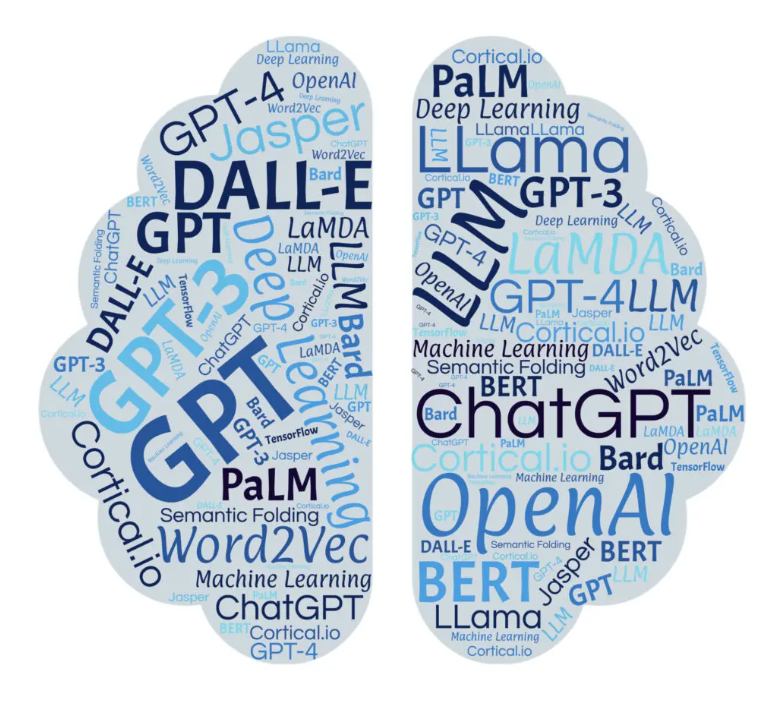
\includegraphics[width=\textwidth]{llm1.png}
            \caption{relevant concepts\footnote{Source: url{https://www.cortical.io/blog/chatgpt-and-large-language-models-the-holy-grail-of-enterprise-ai/}}}
            \label{fig:llm1}
        \end{figure}
    \end{column}
    \begin{column}{0.5\textwidth}
        \begin{itemize}
            \item LLM and AI have become very hot topics in recent years.
            \item Various models have shown their wide usage and significant competence in many fields.
            \item QA, content generation, translation, text classification etc \cite{Liu23}.
        \end{itemize}
    \end{column}
\end{columns}
\end{frame}

\begin{frame}{Background}
  \begin{columns}
    \begin{column}{0.4\textwidth}
        \begin{figure}
            \centering
            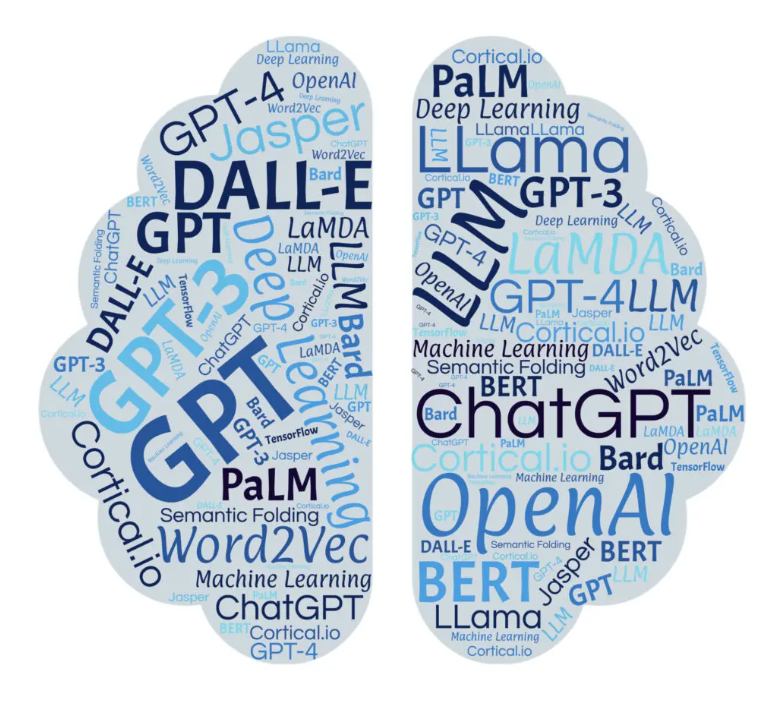
\includegraphics[width=\textwidth]{llm1.png}
            \caption{relevant concepts\footnote{Source: url{https://www.cortical.io/blog/chatgpt-and-large-language-models-the-holy-grail-of-enterprise-ai/}}}
            \label{fig:llm1}
        \end{figure}
    \end{column}
    \begin{column}{0.5\textwidth}
        \begin{itemize}
            \item LLM and AI have become very hot topics in recent years.
            \item Various models have shown their wide usage and significant competence in many fields.
            \item QA, content generation, translation, text classification etc \cite{Liu23}.
            \item Most models are "static" \cite{Gupta23}.
        \end{itemize}
    \end{column}
\end{columns}
\end{frame}

\begin{frame}{Content of the presentation}
  \begin{itemize}
    \item The evolution of language models and the techniques behind them.
    \item The training process of several LLM models.
    \item The definition and application of data streams.
    \item The need, benefits, challenges and use cases of combining LLM with data streams.
  \end{itemize}
\end{frame}
%------------------------------------------------------------------------------------------------------------
\begin{frame}{Large Language Models}
  \vspace{3cm}
  \centering
  \begin{tikzpicture}[
    timeline/.style={
        thick,
        -{Stealth[scale=1.5]},
        line cap=round,
    },
    event/.style={
        circle,
        draw,
        minimum size=6mm,
        fill=blue!20,
        inner sep=0pt,
        font=\footnotesize,
    },
    label/.style={
        font=\small,
        anchor=south,
        text depth=0pt,
    }
]
    % Timeline
    \draw[timeline] (0,0) -- (3,0);
    
    % Events
    \node[event, label=below:{2000}] (event1) at (2,0) {1};
    %\node[event, label=below:{2005}] (event2) at (6,0) {2};
    %\node[event, label=below:{2010}] (event3) at (10,0) {3};
    %\node[event, label=below:{2015}] (event4) at (14,0) {4};
    %\node[event, label=below:{2020}] (event5) at (18,0) {5};
    
    % Event labels
    \node[label, above=of event1] {Statistical Models};
    %\node[label, above=of event2] {Word Embedding};
    %\node[label, above=of event3] {Neural Networks};
    %\node[label, above=of event4] {LSTM};
    %\node[label, above=of event5] {Transformers};
\end{tikzpicture}
\vspace{1cm}
\begin{itemize}
  \item N-Gram \cite{Cavnar94}
  \item Completely statistical.
  \item Calculate the next word's probability based on the N previous sub-words.
  \item Poor performance on large documents.
\end{itemize}
\end{frame}

\begin{frame}{Large Language Models}
  \vspace{3cm}
  \centering
  \begin{tikzpicture}[
    timeline/.style={
        thick,
        -{Stealth[scale=1.5]},
        line cap=round,
    },
    event/.style={
        circle,
        draw,
        minimum size=6mm,
        fill=blue!20,
        inner sep=0pt,
        font=\footnotesize,
    },
    label/.style={
        font=\small,
        anchor=south,
        text depth=0pt,
    }
]
    % Timeline
    \draw[timeline] (0,0) -- (8,0);
    
    % Events
    \node[event, label=below:{2000}] (event1) at (2,0) {1};
    \node[event, label=below:{2005}] (event2) at (6,0) {2};
    %\node[event, label=below:{2010}] (event3) at (10,0) {3};
    %\node[event, label=below:{2015}] (event4) at (14,0) {4};
    %\node[event, label=below:{2020}] (event5) at (18,0) {5};
    
    % Event labels
    \node[label, above=of event1] {Statistical Models};
    \node[label, above=of event2] {Word Embedding};
    %\node[label, above=of event3] {Neural Networks};
    %\node[label, above=of event4] {LSTM};
    %\node[label, above=of event5] {Transformers};
\end{tikzpicture}
\vspace{1cm}
\begin{itemize}
  \item Word2Vec \cite{Mikolov13}
  \item Map words into vector space.
  \item Similar words have a closer distance.
  \item Better performance on large documents.
\end{itemize}
\end{frame}

\begin{frame}{Large Language Models}
  \vspace{3cm}
  \centering
  \begin{tikzpicture}[
    timeline/.style={
        thick,
        -{Stealth[scale=1.5]},
        line cap=round,
    },
    event/.style={
        circle,
        draw,
        minimum size=6mm,
        fill=blue!20,
        inner sep=0pt,
        font=\footnotesize,
    },
    label/.style={
        font=\small,
        anchor=south,
        text depth=0pt,
    }
]
    % Timeline
    \draw[timeline] (0,0) -- (12,0);
    
    % Events
    \node[event, label=below:{2000}] (event1) at (2,0) {1};
    \node[event, label=below:{2005}] (event2) at (6,0) {2};
    \node[event, label=below:{2010}] (event3) at (10,0) {3};
    %\node[event, label=below:{2015}] (event4) at (14,0) {4};
    %\node[event, label=below:{2020}] (event5) at (18,0) {5};
    
    % Event labels
    \node[label, above=of event1] {Statistical Models};
    \node[label, above=of event2] {Word Embedding};
    \node[label, above=of event3] {Neural Networks};
    %\node[label, above=of event4] {LSTM};
    %\node[label, above=of event5] {Transformers};
\end{tikzpicture}
\vspace{1cm}
\begin{itemize}
  \item Seq2Seq \cite{Sutskever14}
  \item Works with Long Short-Term Memory(LSTM).
  \item Encodes input into vectors with fixed dimensionality and decodes them.
  \item Much Better performance on large documents, can work with different input lengths.
  \item But still vanishing gradient problems on very large documents.
\end{itemize}
\end{frame}

\begin{frame}{Large Language Models}
  \vspace{3cm}
  \centering
  \begin{tikzpicture}[
    timeline/.style={
        thick,
        -{Stealth[scale=1.5]},
        line cap=round,
    },
    event/.style={
        circle,
        draw,
        minimum size=6mm,
        fill=blue!20,
        inner sep=0pt,
        font=\footnotesize,
    },
    label/.style={
        font=\small,
        anchor=south,
        text depth=0pt,
    }
]
    % Timeline
    \draw[timeline] (0,0) -- (16,0);
    
    % Events
    \node[event, label=below:{2000}] (event1) at (2,0) {1};
    \node[event, label=below:{2005}] (event2) at (6,0) {2};
    \node[event, label=below:{2010}] (event3) at (10,0) {3};
    %\node[event, label=below:{2015}] (event4) at (14,0) {4};
    \node[event, label=below:{2020}] (event4) at (14,0) {5};
    
    % Event labels
    \node[label, above=of event1] {Statistical Models};
    \node[label, above=of event2] {Word Embedding};
    \node[label, above=of event3] {Neural Networks};
    %\node[label, above=of event4] {LSTM};
    \node[label, above=of event4] {Transformers};
\end{tikzpicture}
\vspace{1cm}
\begin{itemize}
  \item Transformer \cite{Vaswani17}
  \item Works with the self-attention mechanism.
  \item Can process the entire input sentence simultaneously with the help of positional encoding.
  \item Very good performance on large documents, more efficient and powerful.
\end{itemize}
\end{frame}

\begin{frame}{Large Language Models}
  \vspace{3cm}
  \centering
  \begin{tikzpicture}[
    timeline/.style={
        thick,
        -{Stealth[scale=1.5]},
        line cap=round,
    },
    event/.style={
        circle,
        draw,
        minimum size=6mm,
        fill=blue!20,
        inner sep=0pt,
        font=\footnotesize,
    },
    label/.style={
        font=\small,
        anchor=south,
        text depth=0pt,
    }
]
    % Timeline
    \draw[timeline] (0,0) -- (20,0);
    
    % Events
    \node[event, label=below:{2000}] (event1) at (2,0) {1};
    \node[event, label=below:{2005}] (event2) at (6,0) {2};
    \node[event, label=below:{2010}] (event3) at (10,0) {3};
    \node[event, label=below:{2015}] (event4) at (14,0) {4};
    \node[event, label=below:{2020}] (event5) at (18,0) {5};
    
    % Event labels
    \node[label, above=of event1] {Statistical Models};
    \node[label, above=of event2] {Word Embedding};
    \node[label, above=of event3] {Neural Networks};
    \node[label, above=of event4] {Transformers};
    \node[label, above=of event5] {Recent Models};
\end{tikzpicture}
\vspace{1cm}
\begin{itemize}
  \item BERT, ChatGPT, LLaMA\dots
  \item Based on the transformer architecture.
  \item Trained on massive datasets and fine-tuned with downstream tasks.
  %\item Very good performance on large documents, more efficient and powerful.
\end{itemize}
\end{frame}

\section{Training process of LLMs}
\begin{frame}{Tokenization}
  \begin{itemize}
    \item Purpose: Segmenting input text into tokens.
    \item WordPiece (BERT) \cite{Wu16}
    \item Byte Pair Encoding (GPT2, LLaMA) \cite{Sennrich15}
    %\item Sentence Piece (LLaMA)
  \end{itemize}
\end{frame}

\begin{frame}{Pre-training}
Given an unlabeled corpus of tokens $U=\{u_1,...,u_n\}$ as a training dataset, the core idea of the pre-training phase is to 
predict the next token $u_i$ for a sequence $\{u_{i-k},...,u_{i-1}\}$, specifically by maximizing the likelihood: 
\begin{equation}
  L_1(U) = \sum_{i}\log{P(u_i|u_{i-k},...,u_{i-1}; \Theta)} \cite{Radford18}
\end{equation}
$k$ refers to the context window size and $\Theta$ is the parameter of the neural network with which the conditional probability $P$ is modeled.
\end{frame}

\begin{frame}{Fine-tuing}
  Given a labeled dataset $C$,
  where each instance of $C$ has a sequence of tokens \{$c^1,...,c^m$\} and a label $y$, the goal of the fine-tuning phase is to maximize the following likelihood:
  \begin{equation}
    L_2(U) = \sum_{(x,y)}\log{P(y|x^1,...,x^m)} \cite{Radford18}
  \end{equation}
\end{frame}

\begin{frame}{BERT}
  \begin{figure}
    \centering
    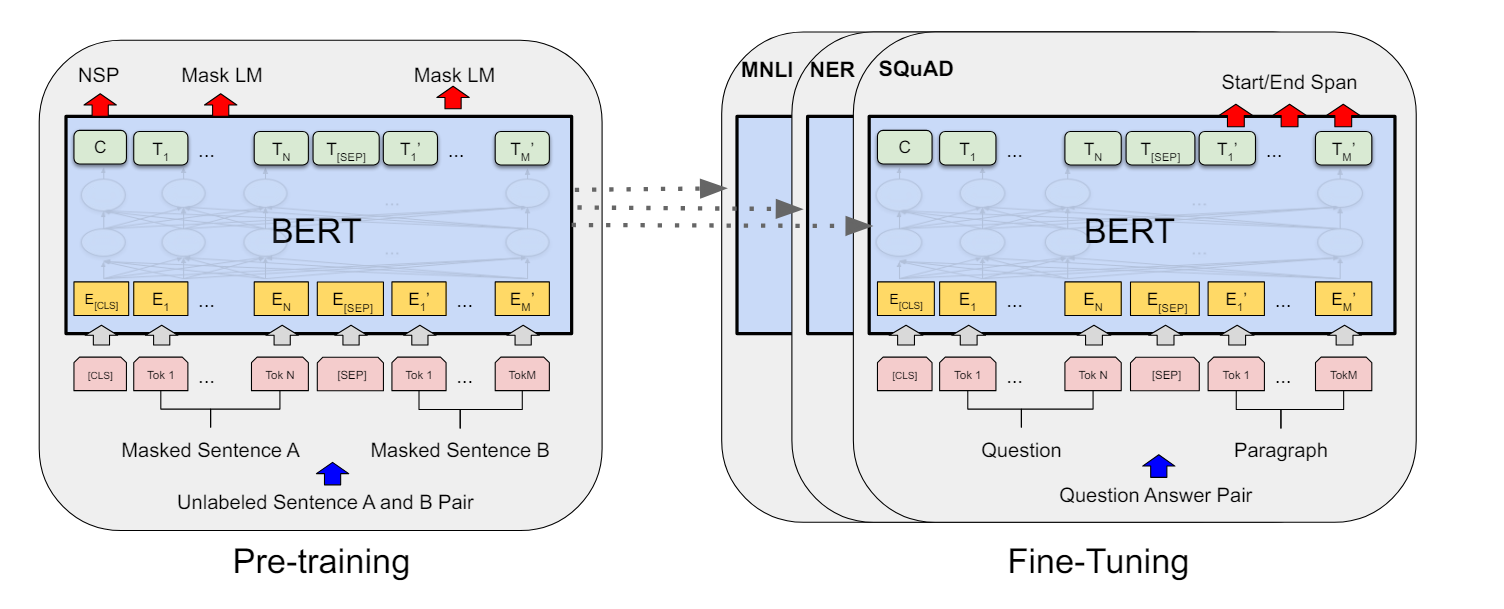
\includegraphics[width=\textwidth]{BERT Finetuning.png}
    \caption{Training Process in the BERT model \cite{Devlin18}}
    \label{fig:llm2}
\end{figure}
\end{frame}

\begin{frame}{A comparison of different models}
  \begin{figure}
    \centering
    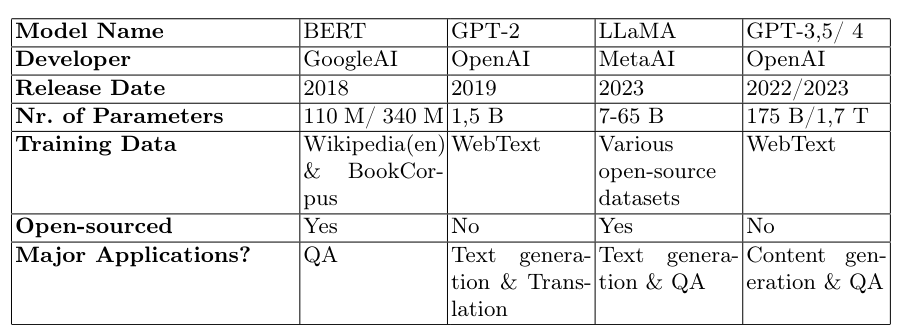
\includegraphics[width=\textwidth]{comparison.png}
    \caption{A comparison of different LLM models}
    \label{fig:llm3}
\end{figure}
\end{frame}

\section{LLM with data streams}
%\subsection{Continual Learning}
\begin{frame}{Data Stream}
  \vspace{1cm}
  \begin{definition}
    A data stream $S$ is an unbounded, potentially infinite multiset of data stream elements $(s,\tau)$, where $\tau \in \mathbb{T}$.
     $\mathbb{T}$ is a timestamp attribute with values from a monotonic, infinite time domain $\mathbb{T}$ with discrete time units. \cite{Geisler13}
  \end{definition}
\end{frame}

\begin{frame}{Limitation of pre-trained LLMs}
  \vspace{1cm}
  \begin{itemize}
    \item Lack of knowledge beyond the scope of their training datasets.
    \item The performance is likely to gradually degrade over time \cite{Shi24}.
    \item Extremely computationally expensive to be re-trained.
    \item Not able to process data streams as input.
  \end{itemize}
\end{frame}

\section{LLMs and data streams}
\begin{frame}{Challenges}
  Application Fields
\end{frame}

%\subsection{Prompt Engineering}
\begin{frame}{Prompt engineering}
  Text goes here
\end{frame}

\begin{frame}{Continual learning}
  Text goes here
\end{frame}

\section{Conclusion}
\begin{frame}{}
  Text goes here
\end{frame}

\section{References}
\begin{frame}{}
\begin{thebibliography}{}
  \bibitem{Liu23}
  Liu, Yiheng, Tianle Han, Siyuan Ma, Jiayue Zhang, Yuanyuan Yang, Jiaming Tian, Hao He et al. "Summary of chatgpt-related research and perspective towards the future of large language models." Meta-Radiology (2023): 100017.

  \bibitem{Gupta23}
  Gupta, Kshitij, Benjamin Thérien, Adam Ibrahim, Mats L. Richter, Quentin Anthony, Eugene Belilovsky, Irina Rish, and Timothée Lesort. "Continual Pre-Training of Large Language Models: How to (re) warm your model?." arXiv preprint arXiv:2308.04014 (2023).

  \bibitem{Cavnar94}
Cavnar, William B., and John M. Trenkle. "N-gram-based text categorization." In Proceedings of SDAIR-94, 3rd annual symposium on document analysis and information retrieval, vol. 161175, p. 14. 1994.

\bibitem{Mikolov13}
Mikolov, Tomas, Ilya Sutskever, Kai Chen, Greg S. Corrado, and Jeff Dean. "Distributed representations of words and phrases and their compositionality." Advances in neural information processing systems 26 (2013).


\end{thebibliography}
\end{frame}

\begin{frame}
  \begin{thebibliography}{}
    \bibitem{Sutskever14}
Sutskever, Ilya, Oriol Vinyals, and Quoc V. Le. "Sequence to sequence learning with neural networks." Advances in neural information processing systems 27 (2014).

\bibitem{Vaswani17}
Vaswani, Ashish, Noam Shazeer, Niki Parmar, Jakob Uszkoreit, Llion Jones, Aidan N. Gomez, Łukasz Kaiser, and Illia Polosukhin. "Attention is all you need." Advances in neural information processing systems 30 (2017).

\bibitem{Devlin18}
Devlin, Jacob, Ming-Wei Chang, Kenton Lee, and Kristina Toutanova. "Bert: Pre-training of deep bidirectional transformers for language understanding." arXiv preprint arXiv:1810.04805 (2018).

\bibitem{Wu16}
Wu, Yonghui, Mike Schuster, Zhifeng Chen, Quoc V. Le, Mohammad Norouzi, Wolfgang Macherey, Maxim Krikun et al. "Google's neural machine translation system: Bridging the gap between human and machine translation." arXiv preprint arXiv:1609.08144 (2016).
  \end{thebibliography}
\end{frame}

\begin{frame}
  \begin{thebibliography}{}
    \bibitem{Sennrich15}
Sennrich, Rico, Barry Haddow, and Alexandra Birch. "Neural machine translation of rare words with subword units." arXiv preprint arXiv:1508.07909 (2015).

\bibitem{Radford18}
Radford, Alec, Karthik Narasimhan, Tim Salimans, and Ilya Sutskever. "Improving language understanding by generative pre-training." (2018).

\bibitem{Geisler13}
Geisler, Sandra. "Data stream management systems." In Dagstuhl Follow-Ups, vol. 5. Schloss Dagstuhl-Leibniz-Zentrum fuer Informatik, 2013.

\bibitem{Shi24}
Shi, Haizhou, Zihao Xu, Hengyi Wang, Weiyi Qin, Wenyuan Wang, Yibin Wang, and Hao Wang. "Continual Learning of Large Language Models: A Comprehensive Survey." arXiv preprint arXiv:2404.16789 (2024).

  \end{thebibliography}
\end{frame}

\end{document}
